% !TeX root = ../main.tex

\chapter{Introduction}\label{chap:1}

\section{TBD} \label{sec:1.1}
    Blah, Blah, Blah, Blah, Blah, Blah, Blah, \cite{kashyap-fbg, smit-awg-review}. 
    Blah, Blah, Blah, Blah, Blah, Blah, Blah, Blah, Blah, Blah, Blah, Blah, Blah, Blah, \cite{smit-awg-review, smit-1stawg, flat-awg-mmi-1, flat-awg-mmi-2, flat-awg-mmi-3, flat-awg-mmi-4, flat-awg-mmi-5, flat-awg-mmi-6, cwdmf-awg-2, flat-awg-horn-1, flat-awg-horn-2, flat-awg-horn-3, flat-awg-sinc-1, flat-awg-sinc-2, flat-awg-sinc-3, flat-awg-sinc-4, flat-awg-sinc-5, wdmf-awg-1, wdmf-awg-2, wdmf-awg-3, wdmf-awg-4, wdmf-awg-5, wdmf-awg-6, wdmf-awg-7, wdmf-eg-1, wdmf-immi, wdmf-mmwg-1, wdmf-all-1, wdmf-wbg-1, wdmf-wbg-2, wdmf-wbg-3, wdmf-ringamzi-1, cwdmf-mmi-1, cwdmf-mmi-2, cwdmf-mmi-3, cwdmf-eg-1, cwdmf-eg-2, cwdmf-eg-3, cwdmf-wbg-1, cwdmf-wbg-2, cwdmf-wbg-3, cwdmf-wbg-4, cwdmf-wbg-5, cwdmf-wbg-6, cwdmf-awgmzi-1, cwdmf-awgmzi-2, cwdmf-awg-1, cwdmf-awg-2, cwdmf-awg-3, cwdmf-awg-4, cwdmf-awg-5, cwdmf-mzi-1, cwdmf-mzi-2, cwdmf-mzi-3, cwdmf-mzi-4, cwdmf-mzi-5, cwdmf-mzi-6, cwdmf-mzi-7, cwdmf-mzi-8, cwdmf-mzi-9, cwdmf-all} 
    have been implemented for desired filtering responses to improve the system. 
    Among these platforms, silicon-on-insulator (SOI) is one of the most promising 
    candidates for photonics integrated circuits (PICs) given the compatibility with complementary metal-oxide-semiconductor (CMOS) 
    lithographic technology and the high maturity as well as low cost for fabrication and mass production. 
    In recent years, 
    Silicon Photonics (SiPh) based on SOI platform has become more and more popular for PICs \cite{hqp-1, icl-2, mdm-2, cwdmf-eg-3, cwdmf-wbg-1, picp-10, adc-1, mdm-1, wdmf-mmwg-1, wdmf-all-1, psr-1, psr-5, mzm-2, mzm-1, pbs-1, pbs-2, pbs-3, psr-2, psr-3, psr-4, wbg-1, wbg-3, cwdmf-mmi-2, cwdmf-all, cwdmf-wbg-2, fec-1, fec-2, fgc-2, wdmf-wbg-3, wdmf-eg-1, flat-awg-mmi-5, wdmf-awg-5, flat-awg-mmi-4, wdmf-awg-1, wdmf-awg-2, cwdmf-eg-1, cwdmf-eg-2, cwdmf-mzi-1, cwdmf-mzi-2, cwdmf-mzi-4, cwdmf-mzi-6, cwdmf-wbg-4, wdmf-awg-4, wdmf-awg-3, TTAWG-p1, TTAWG-p3, flat-awg-sinc-2, awg-fig-3} because of the advantages. 
    
    In this dissertation, two \ur{MUXs/DEMUXs} based on different mechanisms \cite{wdmf-awg-1, wdmf-awg-2, wdmf-awg-3, wdmf-awg-4, wdmf-awg-5, wdmf-awg-6, wdmf-awg-7, wdmf-wbg-1, wdmf-wbg-2, wdmf-wbg-3, cwdmf-awg-1, cwdmf-awg-2, cwdmf-awg-3, cwdmf-awg-4, cwdmf-awg-5, cwdmf-awgmzi-1, cwdmf-awgmzi-2, cwdmf-wbg-1, cwdmf-wbg-2, cwdmf-wbg-3, cwdmf-wbg-4, cwdmf-wbg-5, cwdmf-wbg-6} 
    over the SOI platform are studied and briefly introduced in the following subsections. 

\subsection{Blah, Blah, Blah, Blah} \label{sec:1.1.1}
    \begin{figure}[!h]
		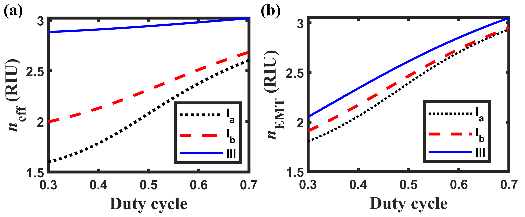
\includegraphics{Fig_sample.pdf}
		\centering
		\caption[Schematic configuration of a conve\ur{n}tional AWG.]
            {\label{fig:1.1}Schematic configuration of a conve\ur{n}tional AWG \cite{awg-fig-2}.}
	\end{figure}
    Blah, Blah, Blah, Blah, Blah, Blah, Blah, Blah, Blah, Blah, Blah, Blah, Blah, Blah, Blah, 
    Blah, Blah, Blah, Blah, Blah, Blah, Blah, Blah, Blah, Blah, Blah, Blah, Blah, Blah, Blah, 
    \begin{figure}[!t]
		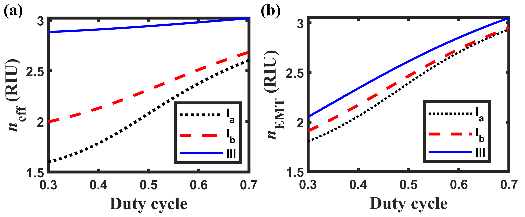
\includegraphics{Fig_sample.pdf}
		\centering
		\caption[Microscope images of an AWG for 1$\times$8 WDM syst\ur{em}]
            {\label{fig:1.2}Microscope images of an AWG for 1$\times$8 WDM syst\ur{em} \cite{awg-fig-2}.}
	\end{figure}
    Blah, Blah, Blah, Blah, Blah, Blah, Blah, Blah, Blah, Blah, Blah, Blah, Blah, Blah, Blah, 
    \begin{figure}[!t]
		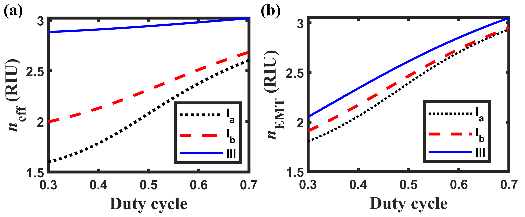
\includegraphics{Fig_sample.pdf}
		\centering
		\caption[SEM images of the AWG shown in Fig.~\ref{fig:1.2}]
            {\label{fig:1.3}SEM images of the AWG shown in Fig.~\ref{fig:1.2} \cite{awg-fig-2}.}
	\end{figure}
    Blah, Blah, Blah, Blah, Blah, Blah, Blah, Blah, Blah, Blah, Blah, Blah, Blah, Blah, Blah, Blah, Blah, Blah, Blah, 
    Blah, Blah, Blah, Blah, Blah, Blah, Blah, Blah, Blah, Blah, Blah, Blah, Blah, Blah, Blah, Blah, Blah, Blah, Blah, 
    Blah, Blah, Blah, Blah, Blah, Blah, Blah, Blah, Blah, Blah, Blah, Blah, Blah, Blah, Blah, Blah, Blah, Blah, Blah, 
    Blah, Blah, Blah, Blah, Blah, Blah, Blah, Blah, Blah, Blah, Blah, Blah, Blah, Blah, Blah, Blah, Blah, Blah, Blah, 
    Blah, Blah, Blah, Blah, Blah, Blah, Blah, Blah, Blah, Blah, Blah, Blah, Blah, Blah, Blah, Blah, Blah, Blah, Blah, 
    Blah, Blah, Blah, Blah, Blah, Blah, Blah, Blah, Blah, Blah, Blah, Blah, Blah, Blah, Blah, Blah, Blah, Blah, Blah.

\subsection{Arrayed waveguide grating (AWG)} \label{sec:1.1.2}
    Blah, Blah, Blah, Blah, Blah, Blah, Blah, Blah, Blah, Blah, Blah, Blah, 
    Blah, Blah, Blah, Blah, Blah, Blah, Blah, Blah, Blah, Blah, Blah, Blah, Blah, Blah, 

% \section{Research motivation and objectives} \label{sec:1.2}

\section{Dissertation configuration} \label{sec:1.2}
    This dissertiation starts with the introduction in Chapter~\ref{chap:1}, illustraing research motivation and objectives. 
    In Chapter~\ref{chap:2}, basic theories for the researches are given, 
    including working principle of AWG (Section~\ref{sec:2.1}), 
    thermal tuning (Section~\ref{sec:2.2}), and WBG (Section~\ref{sec:2.3}).
    For efficient design and analysis of the devices, 
    four solutions including beam propagation method (BPM) (Section~\ref{sec:2.4.1}), 
    heat transport method (Section~\ref{sec:2.4.2}), 
    finite difference eigenmode (FDE) method (Section~\ref{sec:2.4.3}), and 
    finite-difference time-domain (FDTD) method (Section~\ref{sec:2.4.4}) 
    provided by commercial softwares are utilized in the studies, 
    and briefly introduced in the corresponding subsections. 
    
    In Chapter~\ref{chap:3}, 
    a thermally bi-directional tuning feasibility is proposed and demonstrated on an S-shaped AWG 
    at ultra-low voltage using parallel-circuit configuration.
    In Chapter~\ref{chap:4}, 
    a design methodology of WBG is presented to obtain ultra-low XTs and high fabrication tolerance. 
    Moreover, an engineered amplitude apodization based on permittivity-perturbed coupled-mode theory (PPCMT) 
    is employed for accurate evaluation of the resonant wavelength brought by maximum contra-directional coupling coefficient, 
    decreasing the difficulty of designing such devices and the side-lobe imbalance (SLI). 
    At the end of this dissertation, summary and suggestions for future work are given in Chapter~\ref{chap:5}.
